%%%%%%%%%%%%%%%%%%%%%%%%%%%%%%%%%%%%%%%%%%%%%%%%%%%%%%%%%%%%%%%%%%%%%%%%%%%%%%%%%%%%%%%%%%%%%%%%%%%
% Chapter 3 -> Methods
% Author: Mingbo Cheng
%%%%%%%%%%%%%%%%%%%%%%%%%%%%%%%%%%%%%%%%%%%%%%%%%%%%%%%%%%%%%%%%%%%%%%%%%%%%%%%%%%%%%%%%%%%%%%%%%%%
%\addbibresource{~/MEGA/MEGAsync/phd/thesis_Cheng/preamble/thesis.bib}
\chapter{Methods}
\label{chapter:methods}
\graphicspath{{chapter3/figs}}

In the previous chapter, we introduced the concept of profiling the single-cell transcriptome, genome, epigenome, and proteome, along with simultaneous sequencing. We also outlined the common workflow for analyzing single-cell sequencing data from different protocols and that of single-cell multimodal analysis. We discussed the challenges associated with single-cell multimodal integration due to various feature distributions and types. To tackle this, our goal is to develop computational methods to effectively integrate single cells of multiple modalities. Another challenge in single-cell multimodal analysis is inferring a trajectory to capture cell fate differentiation. To address this challenge, we aim to develop a computational trajectory inference method tailored for single-cell multimodal data, particularly in complex datasets.

In this chapter, we exclusively present and formalize our computational solution towards the two goals. Specifically, we divide the chapter into two main parts: single-cell multimodal dimensional integration (\sref{methods:integration}) and trajectory inference \sref{methods:TI}.

In \sref{methods:integration}, we first introduce the notation that is necessary to formalize our methods.

In \sref{methods:TI}, Similarly, we first introduce the notation that is necessary to formalize our methods.


\section{Single cell Multi-modal dimensional integration}
\label{methods:integration}
\subsection{Notation}
$\mathbf{0}_{p\times q}: $ A $p\times q$ block matrix with all zero elements.\\
$I_p:$ a p-dimensional identity matrix.\\
$A^{-\top}:$ the transposed inverse of $A$\\
$A^{1/2}:$ a square root of $A$\\
$A^{-\top/2}:$ the transposed inverse of $A^{-1/2}$\\
$<\mathbf{z}_a, \mathbf{z}_b>:$ the angel between $\mathbf{z}_a$ and $\mathbf{z}_b$

\subsection{Pre-processing and Dimensional reduction}
Our method take dimensional reductions of $m$ modalities count matrices as input, the count matrices can be represented as
\begin{equation}
    \mathcal{X}=\{X_1,X_2,\cdots,X_m\}
\end{equation}
where $X_{i} \in \mathbb{R}^{n\times s_{i}}$ represents the data of a particular single cell modality, $n$ represents the number of cells, and $s_{i}$ represents the number of features in modality $i$. Here, we focus on multimodal data, where the cells are the same across matrices and there is no direct relation between the features of the distinct modalities. To genereate inputs of our method, we process distinct pre-process and next obtain a dimension reduced matrix for each modality independently using a modality-specific approach: 
\begin{align}
    Y_{i}=f_{i}(X_{i})
\end{align}
where $Y_{i} \in \mathbb{R}^{n\times p_{i}}$ represents the low-dimensional matrix for modality $i$, $p_{i}$ represents the number of dimensions and $f_{i}$ represents the specific dimension reduction method for this modality. 

The pre-processing steps for transcriptome, epigenome, and proteome modalities have been detailed in \sref{background:sec2:scRNA}, \sref{background:sec2:scATAC}, and \sref{background:sec2:protein}. We employ widely used methods for pre-processing, including log normalization followed by feature selection for scRNA-seq data, retaining the top 3,000 features and scaling the data. For scATAC-seq data, we apply TF-IDF transformation to the peaks. In the case of surface protein data, a centered log ratio transformation is employed.


To reduce dimensions, we employ latent semantic indexing (LSI) for scATAC-seq and principal component analysis (PCA) for other modalities, following the common practice in the literature~\cite{granja2021archr, signac, hao2021seurat4}. LSI involves applying singular value decomposition (SVD) on the feature matrix of scATAC data, such that:
\begin{equation}
    Y_{j}' = U\Sigma V^\top
\end{equation}
Where $Y_{j}'\in \mathbb{R}^{n\times s_{j}}$ represents the TF-IDF transformed feature matrix, columns of left singular vector $U\in \mathbb{R}^{n\times p_j}$ is the reduced dimensions.  

The rationale behind the use of dimension reduction is two-fold. First, low-dimensional matrices reduce the computing time of the CCA analysis without impacting accuracy for a minimum number of dimensions. Moreover, it allows to work directly on batch-corrected data, which is usually represented in a low-dimensional space~\cite{hao2021seurat4, korsunsky2019harmony}. Of note, batch correction is recommended previous to the integration, whenever the data is affected by batch effects, see \fref{fig:batch_correction}. 

\subsection{Integration}

\subsubsection{Canonical Correlation analysis for two modalities}
Canonical Correlation analysis(CCA) was first introduced H.Hotelling\citep{hotelling1935cca1,HOTELLING1936cca2} as a multivariate statistical methods for the analysis of paired sets of variables. In multivariate statistical analysis, the dataset consists of several variables measured across a group of observations or individuals. In the context of Canonical Correlation Analysis (CCA), the variables for a given observation can be divided into two distinct sets, representing the two perspectives or views of the data. Let the views $a$ and $b$ be denoted by the matrices $\mathbf{Y}_a\in\mathbb{R}^{n\times p}$ and $\mathbf{Y}_b\in \mathbb{R}^{n\times q}$. The row vectors $\mathbf{y}_a^k\in \mathbb{R}^{p}$ and $\mathbf{y}_b^k$ for $k\in\{1,2,\cdots, n\}$ denotes the sets of empirical multivariate observations in $\mathbf{Y}_a$ and $\mathbf{Y}_b$. The observations are presumed to be collectively drawn from a normal multivariate distribution. And the column vectors $a_i\in \mathbb{R}^n$ for $i\in \{1,2,\cdots, p\}$ and $b_j\in \mathbb{R}^n$ for ${j\in \{1,2,\cdots, q\}}$ denote the variable vectors of the n observations respectively. The problem in CCA can be defined to derive the linear relations between the variables in $\mathbf{Y}_a$ and $\mathbf{Y}_b$ such that the linear transformation:
\begin{equation}
\mathbf{Y}_a\mathbf{w}_a=\mathbf{z}_a\quad\text{and}\quad \mathbf{Y}_b\mathbf{w}_b=\mathbf{ z}_b
\end{equation}

where $\mathbf{Y}_a\in \mathbb{R}^{n\times p}$, ${\mathbf w}_a\in\mathbb{R}^p$, ${\mathbf z}_a\in\mathbb{R}^n$  and $\mathbf{Y}_b\in \mathbb{R}^{n\times q}$, $\mathbf{w}_b\in\mathbb{R}^p$, ${\mathbf z}_b\in\mathbb{R}^n$. The matrices $\mathbf{Y}_a$ and $\mathbf{Y}_b$ symbolize linear transformations of positions ${\mathbf w}_a$ and ${\mathbf w}_b$ onto the images ${\mathbf z}_a$ and ${\mathbf z}_b$ within the space $\mathbb{R}^n$. The terms ``canonical weight vectors'' typically describe the positions ${\mathbf w}_a$ and ${\mathbf w}_b$, while the images ${\mathbf z}_a$ and ${\mathbf z}_b$ are often referred to as ``canonical variates''. The cosine of the angle between ${\mathbf z}_a$ and ${\mathbf z}_b$, referred to as the canonical correlation. The aim of Canonical Correlation Analysis (CCA) is to discover two positions, $\mathbf{w}_a \in \mathbb{R}^p$ and $\mathbf{w}_b \in \mathbb{R}^q$, such that, upon linear transformations $\mathbf{Y}_a \in \mathbb{R}^{n\times p}$ and $\mathbf{Y}_b \in \mathbb{R}^{n\times q}$, they are mapped in a manner that maximizes the cosine of the angle between the position vectors of their images, $\mathbf{z}_a \in \mathbb{R}^n$ and $\mathbf{z}_b \in \mathbb{R}^n$. The first canonical correlation which equals $\cos\theta_1$ corresponding the smallest angle such that:
\begin{equation}
\begin{aligned}
&\cos \theta_1 = \underset{{\mathbf z}_a, {\mathbf z}_b \in\mathbb{R}^n}{\max}<{\mathbf z}_a, {\mathbf z}_b> 
			   = \underset{{\mathbf z}_a, {\mathbf z}_b \in\mathbb{R}^n}{\max}
			   		 \frac{\mathbf{z}_a^\top \mathbf{z}_b}{\|\mathbf{z}_a\| \|\mathbf{z}_b\|} \\
&\text{subject to}\quad \|{\mathbf z}_a\|_2=1\quad \|{\mathbf z}_b\|_2=1
\end{aligned}
\end{equation}
Let the maximum be attained by $z_{a}^{(1)}$ and $z_{b}^{(1)}$. The pair of images $z_{a}^{(2)}$ and $z_{b}^{(2)}$, which has the second smallest enclosing angle $\theta_2$, is located in the orthogonal complements of $z_{a}^{(1)}$ and $z_{b}^{(1)}$. The procedure continues until no more pairs are found. Therefore, the $r$ angles $\theta_r \in [0, \frac{\pi}{2}]$ for $r = (1,2,\cdots,q)$ when $p > q$ that can be found are recursively defined by:

\begin{figure}[!ht]
	\centering
	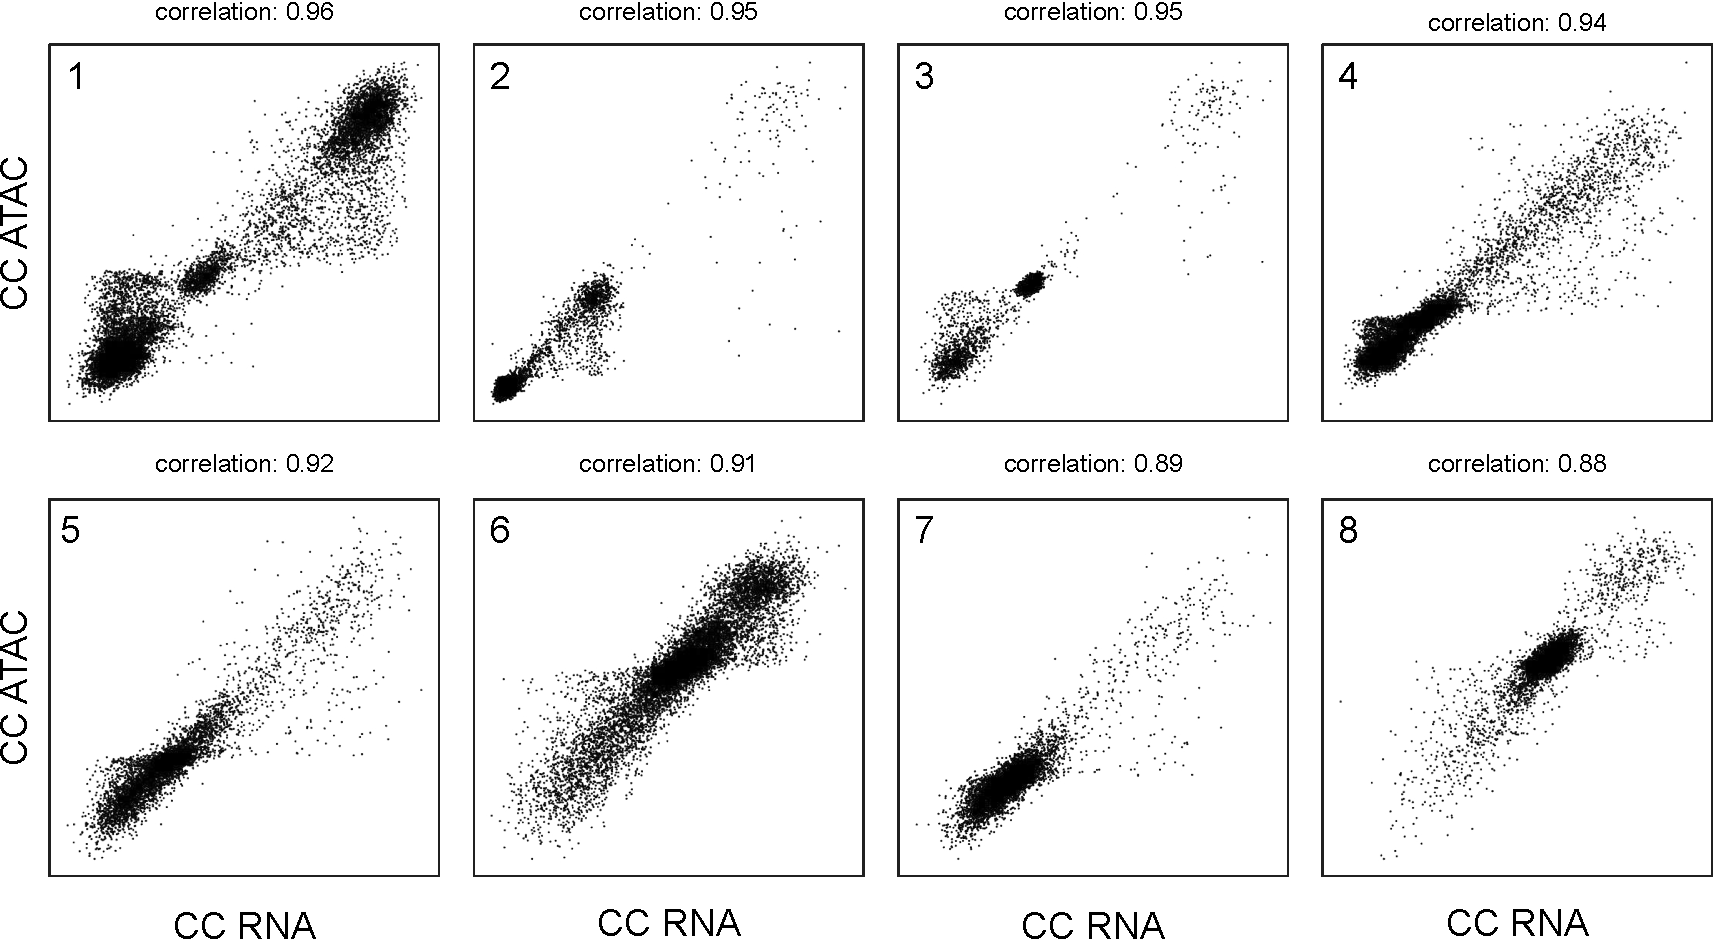
\includegraphics[width=0.95\textwidth]{CC_corrlation_scatter/fig}
	\vspace{0.1cm}
	\caption[Scatter plot illustrating the correlation between scRNA and scATAC.]{\textbf{Scatter plot illustrating the correlation between scRNA and scATAC.} The data is derived from \texttt{PBMC-Multiome}, and the scatter plots depict the highly correlated scRNA and scATAC for the top 8 components. The numbers indicate the $i$-th canonical correlation (CC). The X-axis represents scRNA CC coordinates, while the Y-axis presents the scATAC coordinates.}
	\label{fig:CC_corrlation_scatter}
\end{figure}

\begin{equation}
\begin{aligned}
\cos \theta_r = &\underset{{\mathbf z}_a^r, {\mathbf z}_b^r \in\mathbb{R}^n}{\max}<{\mathbf z}_a^r, {\mathbf z}_b^r>\\
                &\text{subject to  } & \|{\mathbf z}_a\|_2=1\quad \|{\mathbf z}_b\|_2=1\\
				  & & <{\mathbf z}_a^j, {\mathbf z}_a^r>=0\quad <{\mathbf z}_b^j, {\mathbf z}_b^r>=0,\\
				  & & \forall j \neq r: \quad j,r = 1,2,\cdots,\min(p,q).
\end{aligned}
\end{equation}

 To conclude, the essence of Canonical Correlation Analysis (CCA) lies in identifying two positions within their respective data spaces. These positions are chosen such that their images on a unit ball minimize the angle between them, consequently maximizing the canonical correlation. The linear transformations of these positions are governed by the data matrices. The determination of the number of relevant positions can be achieved by analyzing the values of canonical correlations or by applying statistical significance tests.

\begin{figure}[!ht]
	\centering
	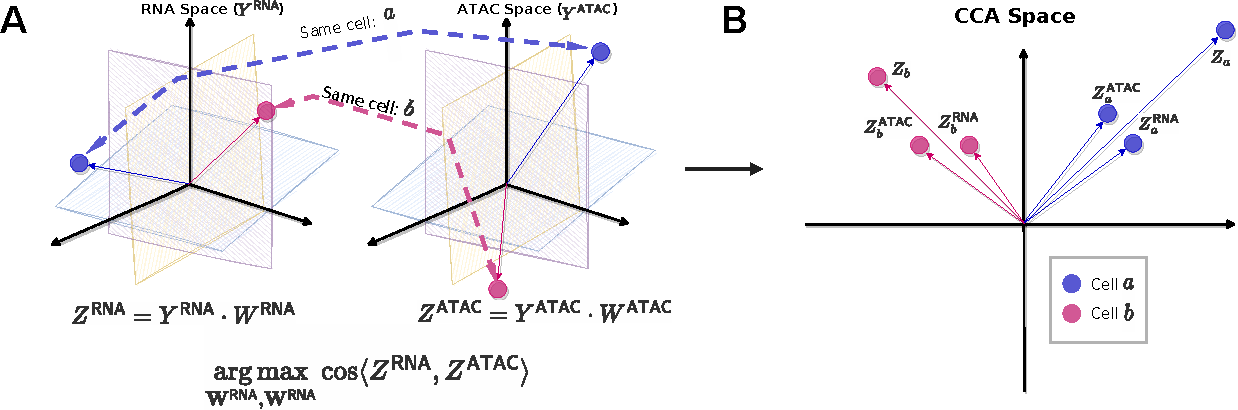
\includegraphics[width=0.95\textwidth]{CCA_ADD/fig}
	\vspace{0.1cm}
	\caption[CCA schematic showing the linear transformation.]{\textbf{CCA schematics illustrating the linear transformation.} The data is sourced from \texttt{PBMC-Multiome}. \textbf{A)} The same cells, denoted as $a$ and $b$, in the scRNA and scATAC space exhibit distinct coordinates. \textbf{B)} Following the linear transformation, cells $a$ and $b$ are projected into the same space with minimized angles. Our approach involves aggregating the two vectors for a cell, resulting in a unified coordinate within the CCA space.}
	\label{fig:CC_pval_select}
\end{figure}

\subsubsection{Solving the Optimization Problem}
There are several ways to solve the CCA problem. The first approach is to apply the standard eigenvalue problem \citep{HOTELLING1936cca2,hooper1959ccaeigen}. It can also be solved by converting it into a generalized eigenvalue problem \citep{bach2002kernel,hardoon2004canonical}. The most commonly used method to solve the problem is by employing Singular Value Decomposition (SVD), first introduced by \citep{healy1957ccasvd}, and further described by \citep{ewerbring1989canonical}. Here, we only introduce the SVD solution, which is applied in our package.
%\citep{HOTELLING1936cca2} shows that we can obtain canonical correlation by solving the  eigendecomposition problem:
%\begin{equation}
%    \det(C_{ab}^\top C_{aa}^{-1} C_{ab} - \lambda C_{bb}) = 0
%\end{equation}
To solve the CCA problem using SVD, we first introduce the joint covariance matrix $C$ such that
\begin{equation}
	C = \begin{pmatrix}
		C_{aa} & C_{ab}\\
		C_{ba} & C_{bb}\\
	\end{pmatrix}	
\end{equation}
Where  and $C_{aa} = \frac{1}{n-1} \mathbf{Y}_a^\top \mathbf{Y}_a$ is the empirical variance matrices between the variables in $\mathbf{Y}_a$, $C_{bb} = \frac{1}{n-1} \mathbf{Y}_b^\top \mathbf{Y}_b$ is the empirical variance matrices between the variables in $\mathbf{Y}_b$ and $C_{ab} = \frac{1}{n-1} \mathbf{Y}_a^\top \mathbf{Y}_b$ is the sample covariance matrix between variable column vectors in $\mathbf{Y}_a$ and $\mathbf{Y}_b$

Next, we reform the CCA problem using the covariance matrices above mentioned. The CCA problem is to find two linear transformations $\mathbf{W}_a$ and $\mathbf{W}_b$ such that:
\begin{equation}
     \mathbf{W}_a^\top C_{aa} \mathbf{W}_a = I_p, \quad  \mathbf{W}_b^\top C_{bb} \mathbf{W}_b = I_q, \quad  \mathbf{W}_a^\top C_{ab}  \mathbf{W}_b = D
\end{equation}
Where $D=\text{diag} (\gamma_i)$, that is:
\begin{equation}
\begin{pmatrix}
     \mathbf{W}_a^\top & {\mathbf 0}\\
    {\mathbf 0} &  \mathbf{W}_b^\top
    \end{pmatrix}
    \begin{pmatrix}
    C_{aa} & C_{ab}\\
    C_{ba} & C_{bb}
    \end{pmatrix}
    \begin{pmatrix}
     \mathbf{W}_a & {\mathbf 0}\\
    {\mathbf 0} &  \mathbf{W}_b
    \end{pmatrix}
    =
    \begin{pmatrix}
    I_p & D\\
    D & I_q
\end{pmatrix}
\end{equation}


We define the canonical variables:
\begin{equation}
    \mathbf{Z}_a= \mathbf{W}_a^\top \mathbf{Y}_a, \quad \mathbf{Z}_b = \mathbf{W}_b^\top \mathbf{Y}_b
\end{equation}

we have a joint covariance matrix
\begin{equation}
    \begin{pmatrix}
    I_p & D \\
    D & I_q
    \end{pmatrix}
\end{equation}
The diagonal elements $\gamma_i$ of D denote the canonical correlations. Thus we find the linear compounds $\mathbf{Z}_a$ and $\mathbf{Z}_b$ to maximize the cross-correlations. 

Since both $C_{aa}$ and $C_{bb}$ are symmetric positive definite, we can perform Cholesky Decomposition on them to get:
\begin{equation}
    C_{aa} = C_{aa}^{\top/2} C_{aa}^{1/2}, \quad C_{bb} = C_{bb}^{\top/2} C_{bb}^{1/2}
\end{equation}

Applying the inverses of the square root factors symmetrically on the joint covariance matrix $C$, the matrix is transformed into:
\begin{equation}
\begin{pmatrix}
    C_{aa}^{-\top/2} & {\mathbf 0}\\
    {\mathbf 0} & C_{bb}^{-\top/2}
    \end{pmatrix}
    \begin{pmatrix}
    C_{aa} & C_{ab}\\
    C_{ba} & C_{bb}
    \end{pmatrix}
    \begin{pmatrix}
    C_{aa}^{-1/2} & {\mathbf 0}\\
    {\mathbf 0} & C_{bb}^{-1/2}
    \end{pmatrix}
    =
    \begin{pmatrix}
    I_p & C_{aa}^{-1/2}C_{ab}C_{bb}^{-1/2}\\
    C_{bb}^{-1/2}C_{ba}C_{aa}^{-1/2} & I_q
\end{pmatrix}
\end{equation}

The canonical correlation problem is reduced to that of finding a SVD of triple product:
\begin{equation}
    U^{\top} (C_{aa}^{-1/2}C_{ab}C_{bb}^{-1/2}) V = D
\end{equation}
The matrix $C$ is thus reduced to the joint covariance matrix such that:
\begin{equation}
    \begin{pmatrix}
        U^\top & {\mathbf 0}\\
        {\mathbf 0} & V^\top
    \end{pmatrix}
    \begin{pmatrix}
        I_p & C_{aa}^{-1/2}C_{ab}C_{bb}^{-1/2}\\
        C_{bb}^{-1/2}C_{ba}C_{aa}^{-1/2} & I_q
    \end{pmatrix}
    \begin{pmatrix}
        U & {\mathbf 0}\\
        {\mathbf 0} & V
    \end{pmatrix} = 
    \begin{pmatrix}
    I_p & D\\
    D^\top & I_q
    \end{pmatrix}
\end{equation}

With the desired transformation $W_a$ and $W_b$:
\begin{equation}
    \mathbf{W}_a = C_{aa}^{-1/2} U, \quad \mathbf{W}_b = C_{bb}^{-1/2}V
\end{equation}
Where the singular values $\gamma_i$ are in descending order such that:
\begin{equation}
    \gamma_1 \geq \gamma_2 \geq \cdots \geq 0    
\end{equation}

The time complexity of CCA for the calculation of $C_{aa}$ and $C_{bb}$ is $O(n\times p \times p)$ and $O(n\times q \times q)$ respectively whereas the time complexity of $C_{ab}$ is $O(n\times p \times q)$. And the time complexity of the  calculation of SVD to solve the problem is $O(\min(p^2q,qp^2))$.

\subsubsection{Uniform latent component}
CCA does not directly provide a unified dimension reduction for single-cell multimodal data. Combining $Z_a$ and $Z_b$ into $q\times 2$ dimensions is not advisable, as a larger dimension increases the risk of the curse of dimensionality. Moreover, correlated components are similar to each other, leading to redundant storage. Additionally, a larger dimensionality negatively impacts the efficiency of downstream analysis. Therefore, we propose a simple method to obtain a unified shared latent space without discarding information from CCA, which involves adding $Z_a$ and $Z_b$ together as follows:
\begin{equation}
    Z = Z_a + Z_b
\end{equation}
Which $Z\in \mathbb{R}^{q}$ is the share latent space. 

\begin{figure}[!ht]
	\centering
	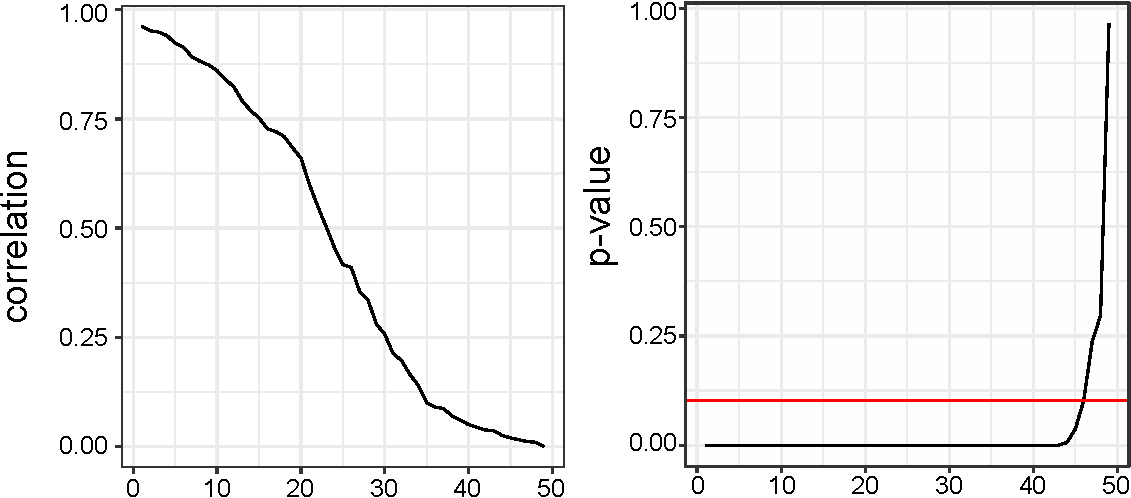
\includegraphics[width=0.95\textwidth]{CC_pval_select/fig}
	\vspace{0.1cm}
	\caption[Line plots showing the CCs correlations and statistics test p-values.]{\textbf{Line plots showing the CCs correlations and statistics test p-values.} Data is from \texttt{PBMC-Multiome}. Left, showing the correlation of scRNA and scATAC CC components from 1 to 49. Right showing the Pearson correlation test outcome from 1 to 49, the red line indicates the significant p-value equals to 0.05}
	\label{fig:CC_pval_select}
\end{figure}

\subsubsection{Selecting the number of components}
Another consideration is whether to retain all components from CCA. Although CCA can calculate as many as $\min(p, q)$ components, not all of them are useful, as the last several components are almost irrelevant, as shown in \fref{fig:CC_corrlations_last}. There are two approaches to select the top components. One method involves examining the correlation of components between two correlation variables. Another approach is to perform a correlation statistical test to exclude unrelated CC pairs, as illustrated in Fig \fref{fig:CC_pval_select}. Our method employs p-values to select correlated components by measuring Pearson correlation and using a student's $t$-test for significance. The $p$-values are then corrected using the BH (Benjamini-Hochberg) method \cite{benjamini1995controlling}, and only canonical components with adjusted p-values < 0.05 are retained.

\subsubsection{Solving Problems with multivariable}
Another issue to be addressed is that conventional CCA cannot handle more than two modalities. Although Multi-CCA has been developed to simultaneously correlate more than 3 variables, it can would probably lead overfitting problem. Thus, we use another way to handle the multimodalities using CCA. For the case that Y has more than two modalities, we perform the pairwise integration of modalities starting with the pair with highest dimensionality. The result of this CCA is then used for integration
with the next modality. See \alref{alg:MOJITOO} for a brief description, which receives a set of matrices $\{Y_{1},\cdots, Y_{m}\}$ with increasing dimensions $p_{i}\geq p_{i+1}$ as input. This heuristic algorithm was adopted to avoid the high computational costs of multiple CCA, which grow exponentially with the number of modalities. 

\subsection{Implementation}
We implemented our Canonical correlation analysis(CCA) based approach to solve the integration of single cell multimodal data as an R package. Our method name is MOJITOO(\textfb{M}ulti-m\textfb{O}dal \textfb{Joint} \textfb{I}ntegra\textfb{T}ion of c\textfb{O}mp\textfb{O}nents) and will be referenced as such throughout this thesis. The method's implementation is all steps as described in this chapter. MOJITOO first was released in January 2022. \fref{fig:MOJITOO_schematic} shows the workflow of MOJITOO and \tref{tab:mojitoo_R_dependencies} summarized the dependencies of MOJITOO package.

\begin{figure}[!ht]
	\centering
	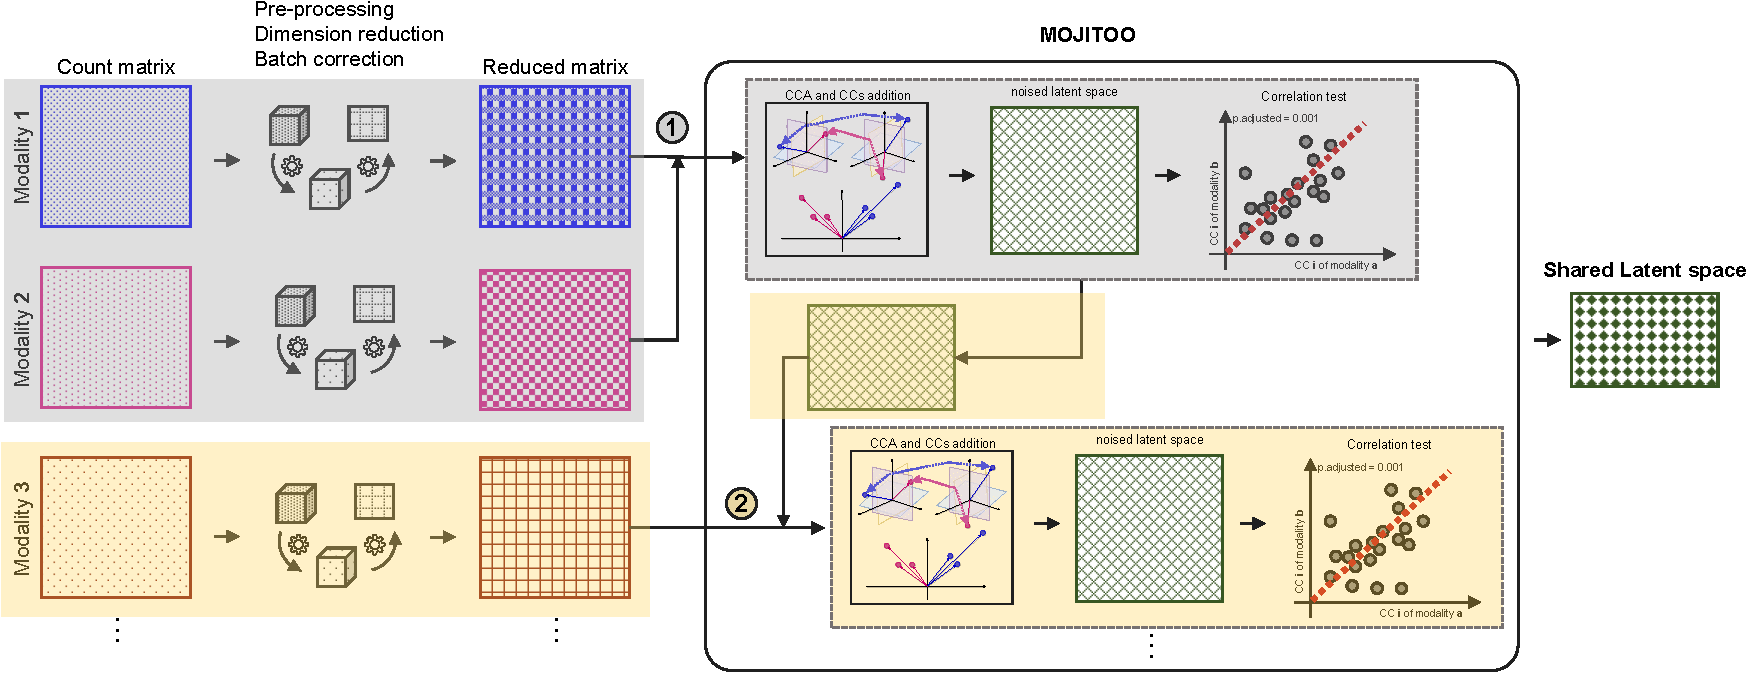
\includegraphics[width=0.95\textwidth]{MOJITOO_schematic/fig}
	\vspace{0.1cm}
	\caption[MOJITOO workflow for multimodal data integration.]{\textbf{MOJITOO workflow for multimodal data integration.} MOJITOO takes dimension reductions of multiple modalities as input. The modalities undergo initial preprocessing, followed by dimension reduction and batch correction if necessary. MOJITOO starts by selecting the two modalities with more features. Subsequently, CCA is employed to correlate the two spaces. The resulting latent spaces are summed to create a shared latent space. A correlation test is then conducted to retain only significant components. The output shared space is iteratively used in the next round of the same operation along with a new modality's dimension reduction. Eventually, the final shared latent space for all modalities is obtained.}
	\label{fig:MOJITOO_schematic}
\end{figure}

MOJITOO requires, at a minimum, a list of dimensional reductions and their specified dimensions as input. The method operates without additional pre-assumption parameters, unless customization of p-value adjusted settings is desired, in which case parameters other than BH (Benjamini-Hochberg) can be adjusted. The integration function `mojitto' accepts any number of dimension reductions, and batch correction for each modality is recommended if needed. MOJITOO outputs a dimension reduction with the default name `mojitoo'.

By default, MOJITOO is designed to work seamlessly with Seurat. It also offers a range of visualization methods for each shared latent component (CC) or for selecting features associated with a specific CC. For CC inspection, `GeneCCDimPlot' generates a UMAP scatter plot of CCs, enabling a detailed examination of each component in the UMAP. `ClusterCCViolin' creates a violin plot for each cluster to visualize CC distribution. For selecting the top positive or negative features, MOJITOO employs `GeneCCHeatmap' to display the top features, such as gene expression, peaks, and transcription factors. Additionally, `ATACTrack' generates genome browser tracks to inspect peaks in each cluster.

Furthermore, MOJITOO is compatible with the widely-used scATAC-seq analysis tool ArchR and has implemented a set of functions for retrieving and setting count matrices, dimensional reduction, and metadata from both Seurat and ArchR. Additionally, for those who prefer Python, we have also implemented a simple Python version that is compatible with popular Python tools like Scanpy and EpiScanpy.

To ensure users utilize MOJITOO correctly, we have provided separate R Markdown vignettes to illustrate how to use MOJITOO with Seurat (\url{https://github.com/CostaLab/MOJITOO/blob/main/vignettes/SeuratObject_integration.Rmd}) and ArchR (\url{https://github.com/CostaLab/MOJITOO/blob/main/vignettes/ArchRObject_integration.Rmd}). Additionally, we have deployed a website listing the MOJITOO API and vignettes at \url{https://costalab.github.io/MOJITOO/index.html}. For Python users, the source code and a simple example are illustrated here: \url{https://github.com/CostaLab/MOJITOO/tree/main/pymojitoo}.
\begin{table}[!ht]
	\centering
	\begin{tabular}{lll}
		\toprule
		\textbf{Package} & \textbf{Version} & \textbf{Website} \\
		\midrule
		  Rcpp  & >= 1.0.7& \url{} \\
		  Seurat & >= 3.2.3 & \url{} \\
		  Signac & >= 1.0.0& \url{} \\
		  reticulate & >= 1.22& \url{} \\
		  corpcor & >= 1.6.10 & \url{} \\
		  S4Vectors & >= 0.30.2 & \url{} \\
		  ramify & >= 0.3.3 & \url{} \\
		  plyr & >= 1.8.6 & \url{} \\
		  rhdf5 & >= 2.36.0 & \url{} \\
		  Matrix & >= 1.3-4 & \url{} \\
		  glue & >= 1.4.2 & \url{} \\
		  dplyr & >= 1.0.7 & \url{} \\
		  reshape2 & >= 1.4.4 & \url{} \\
		  pbapply & >= 1.5-0 & \url{} \\
		  ggplot2 & >= 3.3.5 & \url{} \\
		  ComplexHeatmap & >= 2.11.1 & \url{} \\
		  patchwork & >= 1.1.1 & \url{} \\
		  Gviz & >= 1.36.2 & \url{} \\
		  grid & >= 4.1.0 & \url{} \\
		  tidyr & >= 1.1.4 & \url{} \\
		  fda & >= 5.5.1 & \url{} \\
		  assertthat & >= 0.2.1 & \url{} \\
		\bottomrule
	\end{tabular}
	\vspace{0.1cm}
	\caption[MOJITOO tool R package dependencies]{MOJITOO tool R package dependencies.}
	\label{tab:mojitoo_R_dependencies}
\end{table}

We have tested MOJITOO with R 4.0-4.3 with Rcpp 1.0.7, Seurat 3.2.3,  Signac 1.0.0, reticulate 1.22, corpcor 1.6.10,  S4Vectors 0.30.2,  ramify 0.3.3,  plyr 1.8.6,  rhdf5 2.36.0,  Matrix 1.3-4,  glue 1.4.2,  dplyr 1.0.7,  reshape2 1.4.4,  pbapply 1.5-0,  ggplot2 3.3.5, ComplexHeatmap 2.11.1, patchwork 1.1.1, Gviz 1.36.2, grid 4.1.0, tidyr 1.1.4, fda 5.5.1, and assertthat 0.2.1. We have also tested Python version(3.8-3.10) with numpy 1.23.5, sklearn 1.1.2, scipy 1.10.1, statsmodels 0.14.0, scanpy 1.9.3, and anndata 0.9.2.

We used a local Linux Mint 21.1 x86\_64 64-bit machine running with 12 Intel(R) Core(TM) i5-10400 CPU at 2.90GHz and 64 GB RAM. Moreover, we ran MOJITOO on a High-Performance Computing (HPC) cluster mainly based on AMD EPYC 7452 64-bit nodes at 2.35 GHz and 500 GB RAM with  Rocky Linux 8.9. 

For more information about MOJITOO implementation, source code, tutorials and examples, please see:
\begin{center}
https://github.com/CostaLab/MOJITOO
\end{center}



\begin{algorithm}
	\Input{
	$Y^{(1)},...,Y^{(m)}$
	}

	$i \gets 2$ \\
	$Z^{(1)} \gets Y^{(1)}$ \\
	\While{$i < m$}
	{
		$W^{(1)}, W^{(2)} \gets CCA(Z^{(1)}, Y^{(i)})$ \\ 
		$Z^{(1)} \gets Z^{(1)}\times W^{(1)}$ \\ 
		$Z^{(2)} \gets Y^{(i)}\times W^{(2)}$  \\
		$Z \gets Z^{(1)} + Z^{(2)}$ \\ 
		$Z \gets Z[, 1:k]$\Comment{only consider significantly correlated dimension } 
		$Z^{(1)} \gets Z$ \\
		$i \gets i+1$  \\
	}
	\Return $\mathbf{Z}$ 
	\caption{Multimodal MOJITOO Algorithm }
	\label{alg:MOJITOO}
\end{algorithm}

\subsection{Discussion}
\begin{itemize}

    \item We developed an integration approach through Canonical Correlation Analysis (CCA). We use the Pearson statistical test to select correlated components. Moreover, we add the correlated components not only to obtain a unified latent space but also to avoid higher dimensions, which could potentially cause the curse of dimensionality \citep{Dreyfus2003}. The latent space can be used for downstream analyses such as clustering, trajectory inference, visualization, etc.


    \item The method we propose does not require consideration of feature types. Furthermore, the method takes dimensional reduction inputs from each modality, providing opportunities to apply customized batch correction methods, making it flexible for both modalities and batch correction methods.

    \item Our method is implemented in R and is compatible with popular single-cell analysis toolkits such as Seurat and ArchR. We have provided a tutorial demonstrating how to apply our method to integrate multimodal data using Seurat \url{https://github.com/CostaLab/MOJITOO/blob/main/vignettes/SeuratObject_integration.Rmd} and ArchR \url{https://github.com/CostaLab/MOJITOO/blob/main/vignettes/ArchRObject_integration.Rmd}. Additionally, we have implemented a simple Python version for users collaborating with scanpy or episcanpy \url{https://github.com/CostaLab/MOJITOO/tree/main/pymojitoo}.
\end{itemize}

When examining the concepts behind these single-cell multimodal integration methods, canonical correlation analysis (CCA) is a linear method designed to preserve the maximum amount of information from the original dataset. Other approaches, matrix factorization, such as MOFA, scAI, and Liger, is widely employed due to its intuitive matrix multiplication representations. However, matrix factorization poses a non-convex optimization challenge and may be susceptible to a significant drawback wherein the solution exhibits bias towards one of the optimization variables.

Methods like Seurat WNN generate intricate weighted nearest neighbors networks to capture inter-modality similarities. Nevertheless, this method treats the contribution of each modality equally to derive the final network. In contrast, Schema employs metric learning to reweigh each modality by maximizing the similarity of distance pairs from each modality. However, this approach distorts the distribution of the original data, delivering suboptimal results, and incurs high computational costs owing to its reliance on quadratic programming.

Certain methodologies, such as DIABLO and Symphony, have explored the concept of maximizing covariance or correlation between two modalities. However, the primary use of DIABLO involves employing PLS-DA in a supervised manner for bulk data, where sample labels contribute to the optimization problem. Additionally, DIABLO inputs the original count matrix, leading to remarkably expensive time and memory usage. Symphony serves as a label-transfer method, utilizing canonical correlation analysis for identifying shared references in single-case studies with single-cell CITE-seq data. Nevertheless, Symphony does not incorporate dimension reduction as input, lacks the capability to handle more than two modalities, and employs a suboptimal approach to batch correction removal.

\section{Single cell trajectory inference}
\label{methods:TI}

%a table shows the R dependencies
\subsubsection{trajectory inference}
\begin{figure}[!ht]
	\centering
	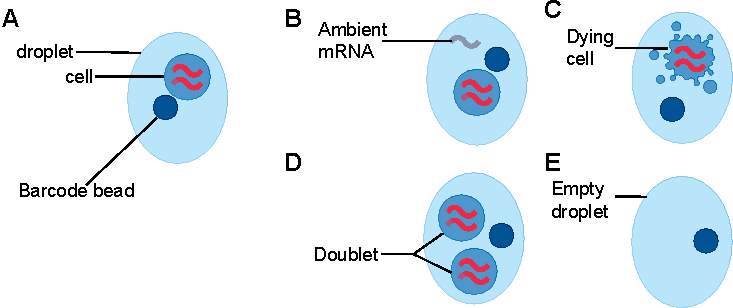
\includegraphics[width=0.95\textwidth]{PHLOWER_schematic/fig}
	\vspace{0.1cm}
	\caption[PHLOWER\_schematic.]{PHLOWER\_schematic}
	\label{fig:PHLOWER_schematic}
\end{figure}

% python package dependencies
\begin{table}[!ht]
	\centering
	\begin{tabular}{lll}
		\toprule
		\textbf{Package} & \textbf{Version} & \textbf{Website} \\
		\midrule
			numpy& >=1.23.5 & \url{https://numpy.org/} \\
			matplotlib& >=3.6.0 & \url{https://matplotlib.org/} \\
			seaborn& >=0.12.0 & \url{https://seaborn.pydata.org/} \\
			pydot& >=1.4.2 & \url{https://github.com/pydot/pydot} \\
			igraph& >=0.10.5 & \url{https://igraph.org/python/} \\
			scikit-learn& >=1.1.2 & \url{https://scikit-learn.org/stable/} \\
			scipy& >=1.10.1 & \url{https://www.scipy.org/} \\
			pandas& >=1.3.5 & \url{https://pandas.pydata.org/} \\
			plotly& >=5.13.1 & \url{https://plotly.com/} \\
			tqdm& >=4.64.1 & \url{https://github.com/tqdm/tqdm} \\
			leidenalg& >=0.9.1 & \url{https://github.com/vtraag/leidenalg} \\
			%louvain& >=0.8.0 & \url{} \\
			colorcet& >=3.0.1 & \url{https://github.com/holoviz/colorcet} \\
			umap-learn& >=0.5.3 & \url{https://github.com/lmcinnes/umap} \\
			scikit-sparse& >=0.4.8 & \url{https://github.com/scikit-sparse/scikit-sparse} \\
			scanpy& >=1.9.3 & \url{https://github.com/scverse/scanpy} \\
			anndata& >=0.8.0 & \url{https://github.com/scverse/anndata} \\
		\bottomrule
	\end{tabular}
	\vspace{0.1cm}
	\caption[PHLOWER tool python package dependencies]{PHLOWER tool python package dependencies.}
	\label{tab:phlower_python_dependencies}
\end{table}
% a table shows the python dependencies
% check how to rotate the title text of a table, see Li's table 3.2
\subsection{Discussion}
